\documentclass[11pt]{article}
\usepackage[margin=0.72in]{geometry}
\usepackage{xcolor}
\usepackage{pagecolor}
\usepackage{graphicx}
\usepackage{booktabs}
\usepackage{amsmath,amssymb}
\usepackage{tcolorbox}
\usepackage{titlesec}
\usepackage[hidelinks]{hyperref}
\usepackage{multicol}

% Bioluminescent Cyber-Editorial Dark Palette
\definecolor{obsidian}{HTML}{07090E}
\definecolor{panelbg}{HTML}{101622}
\definecolor{ink}{HTML}{E2E8F0}
\definecolor{muted}{HTML}{94A3B8}
\definecolor{emerald}{HTML}{00F5A8}
\definecolor{crimson}{HTML}{FF3B5C}
\definecolor{cobalt}{HTML}{3B82F6}
\definecolor{amber}{HTML}{FFB800}
\definecolor{violet}{HTML}{C084FC}

\pagecolor{obsidian}
\color{ink}
\setlength{\parindent}{0pt}
\setlength{\parskip}{7pt}

\titleformat{\section}{\Large\bfseries\sffamily\color{emerald}}{\thesection\ //}{0.5em}{}[\color{emerald}\titlerule]
\titleformat{\subsection}{\large\bfseries\sffamily\color{amber}}{\thesubsection}{0.5em}{}

\newtcolorbox{monolith}[2][emerald]{
  colback=panelbg,
  colframe=#1,
  coltitle=obsidian,
  colupper=ink,
  fonttitle=\bfseries\sffamily\small,
  title=#2,
  arc=4pt,
  boxrule=1.2pt,
  left=10pt,right=10pt,top=8pt,bottom=8pt
}

\newtcolorbox{pullquote}{
  colback=panelbg,
  colframe=crimson,
  leftrule=4pt,rightrule=0pt,toprule=0pt,bottomrule=0pt,
  arc=0pt,
  left=12pt,right=10pt,top=8pt,bottom=8pt
}

\begin{document}
\thispagestyle{empty}

% === FULL-BLEED EDITORIAL COVER HEADER ===
\noindent{\color{emerald}\rule{\textwidth}{3pt}}
\vspace{8pt}

{\sffamily\footnotesize\bfseries\color{crimson} SPECIAL DISPATCH // COMPUTATIONAL PHARMACOLOGY // 2015 $\longrightarrow$ 2026}

\vspace{6pt}
{\sffamily\Huge\bfseries\color{white} WE BURIED A TEN-YEAR-OLD THESIS UNDER 1,000 MODELS IN ONE AFTERNOON.}

\vspace{10pt}
{\large\color{muted} \emph{An unhinged (yet p-value-verified) autopsy of what eleven years of open-source chemistry, cloud GPUs, 77-million-molecule language models, and AI research orchestration just did to a 2015 Cytochrome P450 master's thesis.}}

\vspace{8pt}
{\sffamily\small\color{ink} \textbf{Daniel E.\ Siegle} \quad\color{muted}| \quad M.S.\ Thesis Extension (NCCU 2015 $\to$ 2026) \quad | \quad Total GPU Spend: \textbf{\color{emerald}1.80 Colab Compute Units}}

\vspace{12pt}
% KPI STRIP
\begin{tabular*}{\textwidth}{@{\extracolsep{\fill}}cccc}
\begin{minipage}[t]{0.23\textwidth}\begin{monolith}[emerald]{MEAN TEST AUC}
{\Huge\bfseries\sffamily\color{white} 0.8792}\\[2pt]
{\scriptsize\color{emerald} +0.0375 vs 2015 SVM}\\
{\scriptsize\color{muted} $p \le 2.7\!\times\!10^{-7}$ (5/5)}
\end{monolith}\end{minipage}
&
\begin{minipage}[t]{0.23\textwidth}\begin{monolith}[cobalt]{MEAN TEST ACC}
{\Huge\bfseries\sffamily\color{white} 80.63\%}\\[2pt]
{\scriptsize\color{cobalt} +4.23\% vs 2015 SVM}\\
{\scriptsize\color{muted} +6.50\% vs 2015 RF}
\end{monolith}\end{minipage}
&
\begin{minipage}[t]{0.23\textwidth}\begin{monolith}[violet]{ZERO-MOE AUC}
{\Huge\bfseries\sffamily\color{white} 0.8777}\\[2pt]
{\scriptsize\color{violet} 100\% Open-Source}\\
{\scriptsize\color{muted} MOE lift = ns (5/5!)}
\end{monolith}\end{minipage}
&
\begin{minipage}[t]{0.23\textwidth}\begin{monolith}[crimson]{WALL-CLOCK}
{\Huge\bfseries\sffamily\color{white} 3.5 hrs}\\[2pt]
{\scriptsize\color{crimson} AI-Orchestrated}\\
{\scriptsize\color{muted} vs 2--3 semesters (2015)}
\end{monolith}\end{minipage}
\end{tabular*}

\vspace{10pt}
\begin{pullquote}
{\large\itshape\color{white} ``In 2015, a single-vCPU AWS Free Tier micro instance wheezed at 10\% CPU credits overnight to prove open-source learners could beat MOE Binary QSAR. In 2026, we ran 30 architectures, 150 multi-task neural nets, 50 graph networks, and 25 fine-tuned 77M-molecule transformers on the exact same test sets before dinner---and proved proprietary MOE descriptors are now statistically indistinguishable from zero.''}
\end{pullquote}

\begin{multicols}{2}
\section{The Crime Scene (2015)}
Eleven years ago, my master's thesis at North Carolina Central University asked a scrappy, pragmatic question: could free Python classifiers beat the proprietary Molecular Operating Environment (MOE) Binary QSAR model at predicting whether small molecules inhibit the five major drug-metabolizing cytochrome P450 isozymes (1A2, 2C9, 2C19, 2D6, 3A4) in PubChem AID1851?

They could---and they did, on every single isozyme. But look closely at the 2015 battlefield: we were still \emph{renting MOE's eyeballs} (186 proprietary 2D descriptors), running single-task models in isolation, skipping formal statistical tests, and watching AWS Free Tier \texttt{t1.micro}/\texttt{t2.micro} instances (1 vCPU, 613\,MiB--1\,GiB RAM, throttled to a brutal 10\% baseline CPU once burst credits evaporated after 30 minutes) grind through RBF-SVM folds overnight or for days. And behind those notebooks were 2--3 semesters of simultaneously learning Python, Linux CLI, EC2, \LaTeX, MOE, cheminformatics, and graduate Pharmaceutical Sciences.

\section{The Controlled Experiment}
Almost nobody in machine learning ever gets a clean eleven-year longitudinal control. We did. We locked the \textbf{exact 2015 Figshare training and test CSVs}, locked the $\text{ActivityScore} \ge 40$ threshold, refused to drop even the 0.13\% of compounds missing SMILES (\textbf{100\% test coverage}), and erected a programmatic double-firewall guaranteeing \textbf{zero cross-isozyme test or validation leakage} across all five CYP heads.

\section{The Autopsy of +0.0375 AUC}
Hype says ``deep learning ate everything.'' The data says something far cooler:
\begin{itemize}
  \item \textbf{\color{cobalt}52\% (+0.0196 AUC) came from modern tabular math on unchanged 2015 MOE columns.} LightGBM, XGBoost, CatBoost, QuantileTransformer, and nested stacking did half the decade's work without a single new feature.
  \item \textbf{\color{amber}37\% (+0.0138 AUC) came from open-source RDKit chemistry.} Morgan count FPs, pharmacophore bits, MACCS keys, RDKit 2D descriptors, and exact Tanimoto/Hybrid kernels crushed MOE-only stacks---and held up \emph{better} under strict Bemis--Murcko scaffold splitting ($-0.0100$ vs $-0.0104$ drop).
  \item \textbf{\color{crimson}11\% (+0.0042 AUC, $p<0.03$ on 5/5) came from GPU multi-task deep learning and pretrained SMILES transformers.} On data-scarce CYP 2D6 ($N=4{,}433$), a single 5-head Multi-Task ResMLP jumped to \textbf{80.07\%} accuracy, and \texttt{ChemBERTa-77M-MTR} read \emph{raw SMILES strings} (zero descriptors!) to beat the entire 186-MOE Tier 1 ensemble (0.8659 vs 0.8612 AUC).
\end{itemize}
\end{multicols}

\newpage
\section{The Evidence Plates}

\begin{center}
\fcolorbox{emerald}{white}{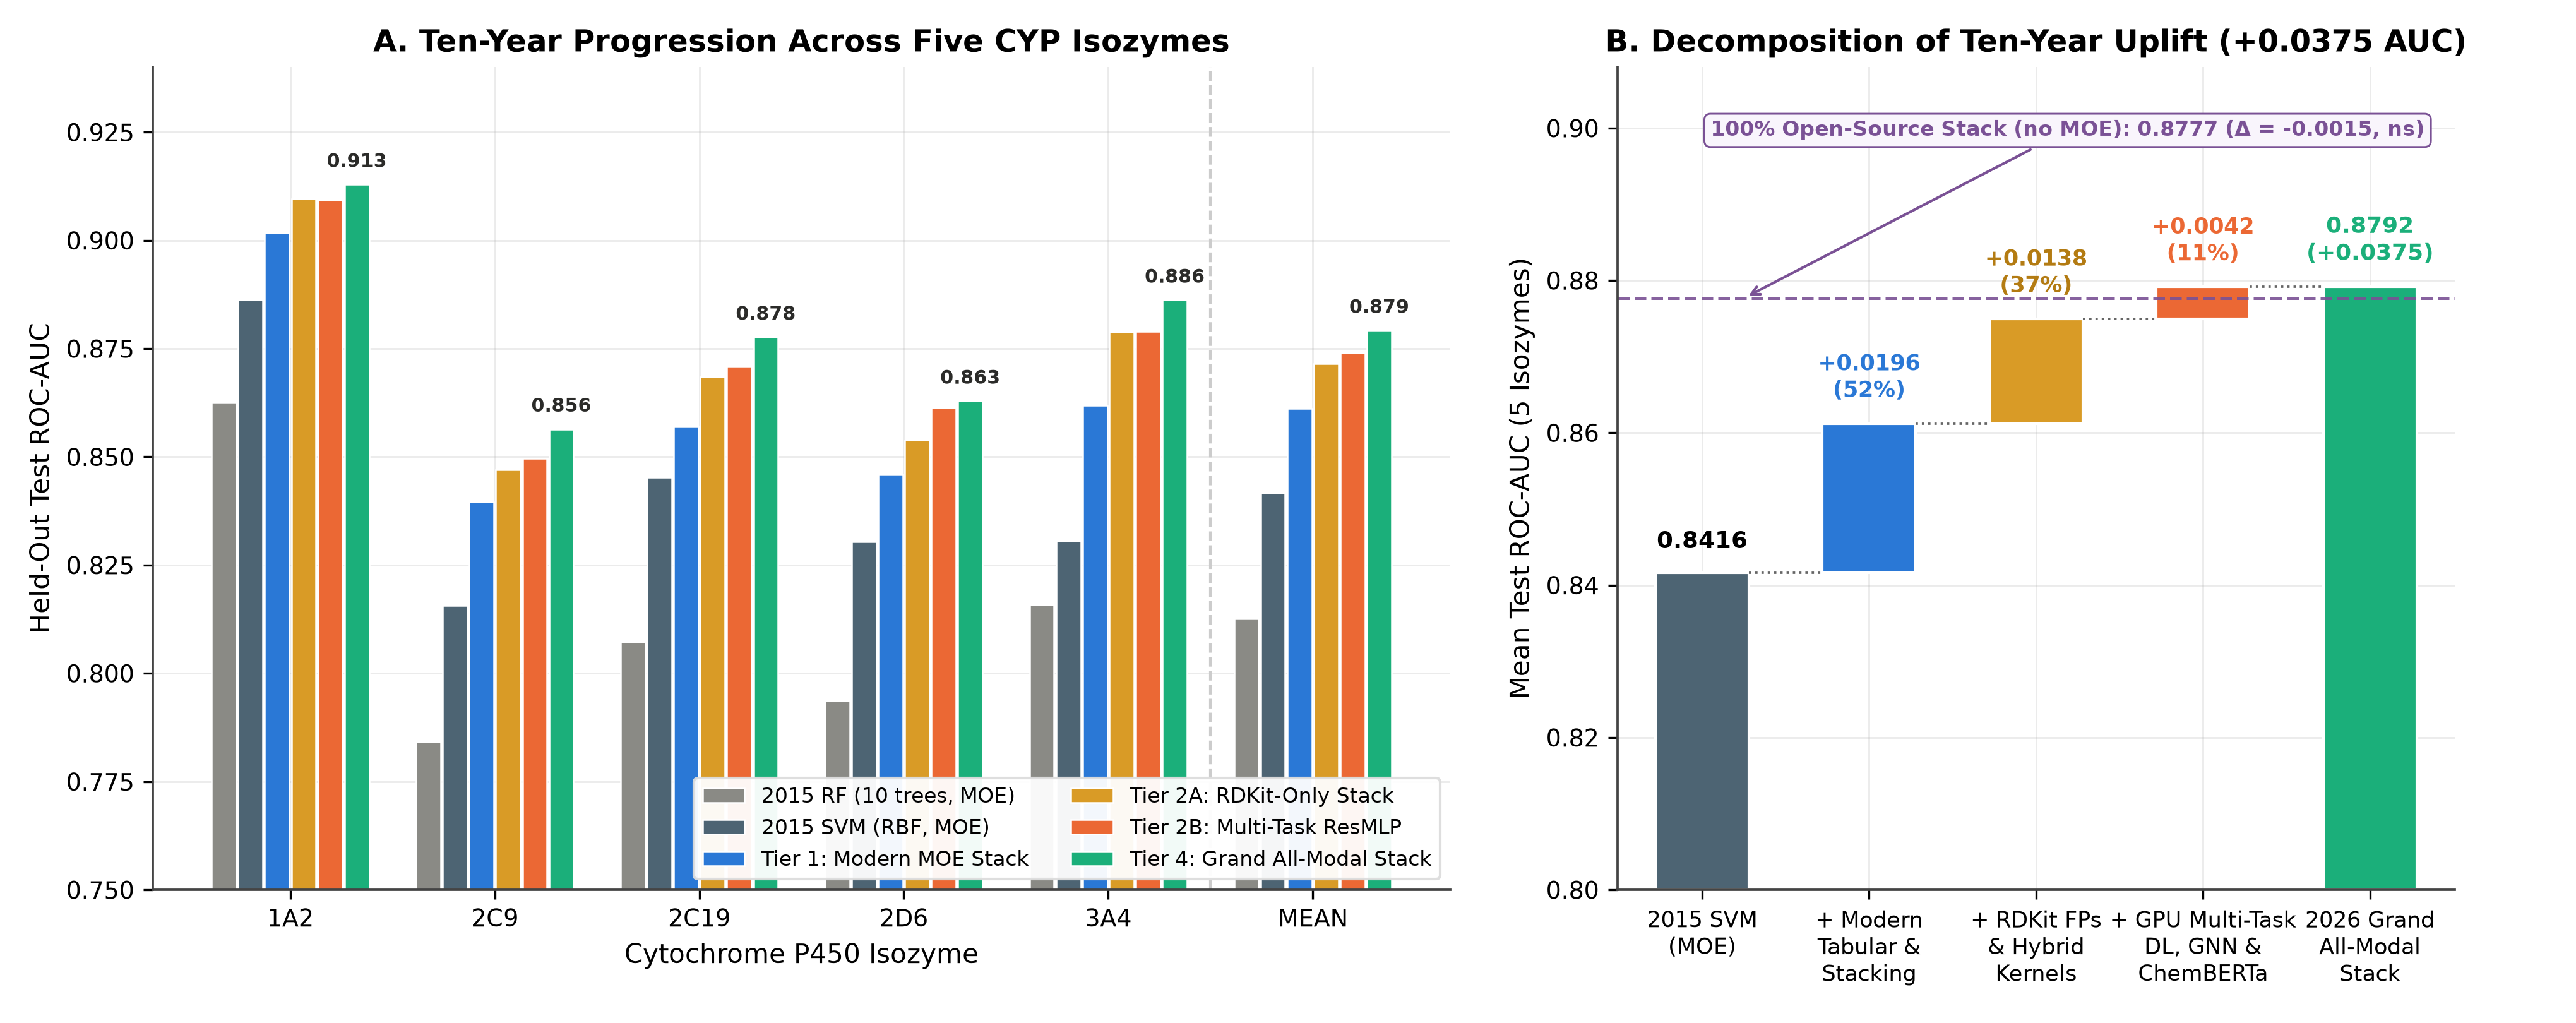
\includegraphics[width=0.96\textwidth]{../img/fig1_ten_year_progression.png}}\\[4pt]
{\scriptsize\sffamily\color{muted}\textbf{PLATE 1.} Ten-year Test ROC-AUC progression and exact uplift waterfall (+52\% tabular math, +37\% RDKit chemistry, +11\% GPU multi-task DL/GNN/ChemBERTa).}
\end{center}

\vspace{8pt}
\begin{center}
\fcolorbox{crimson}{white}{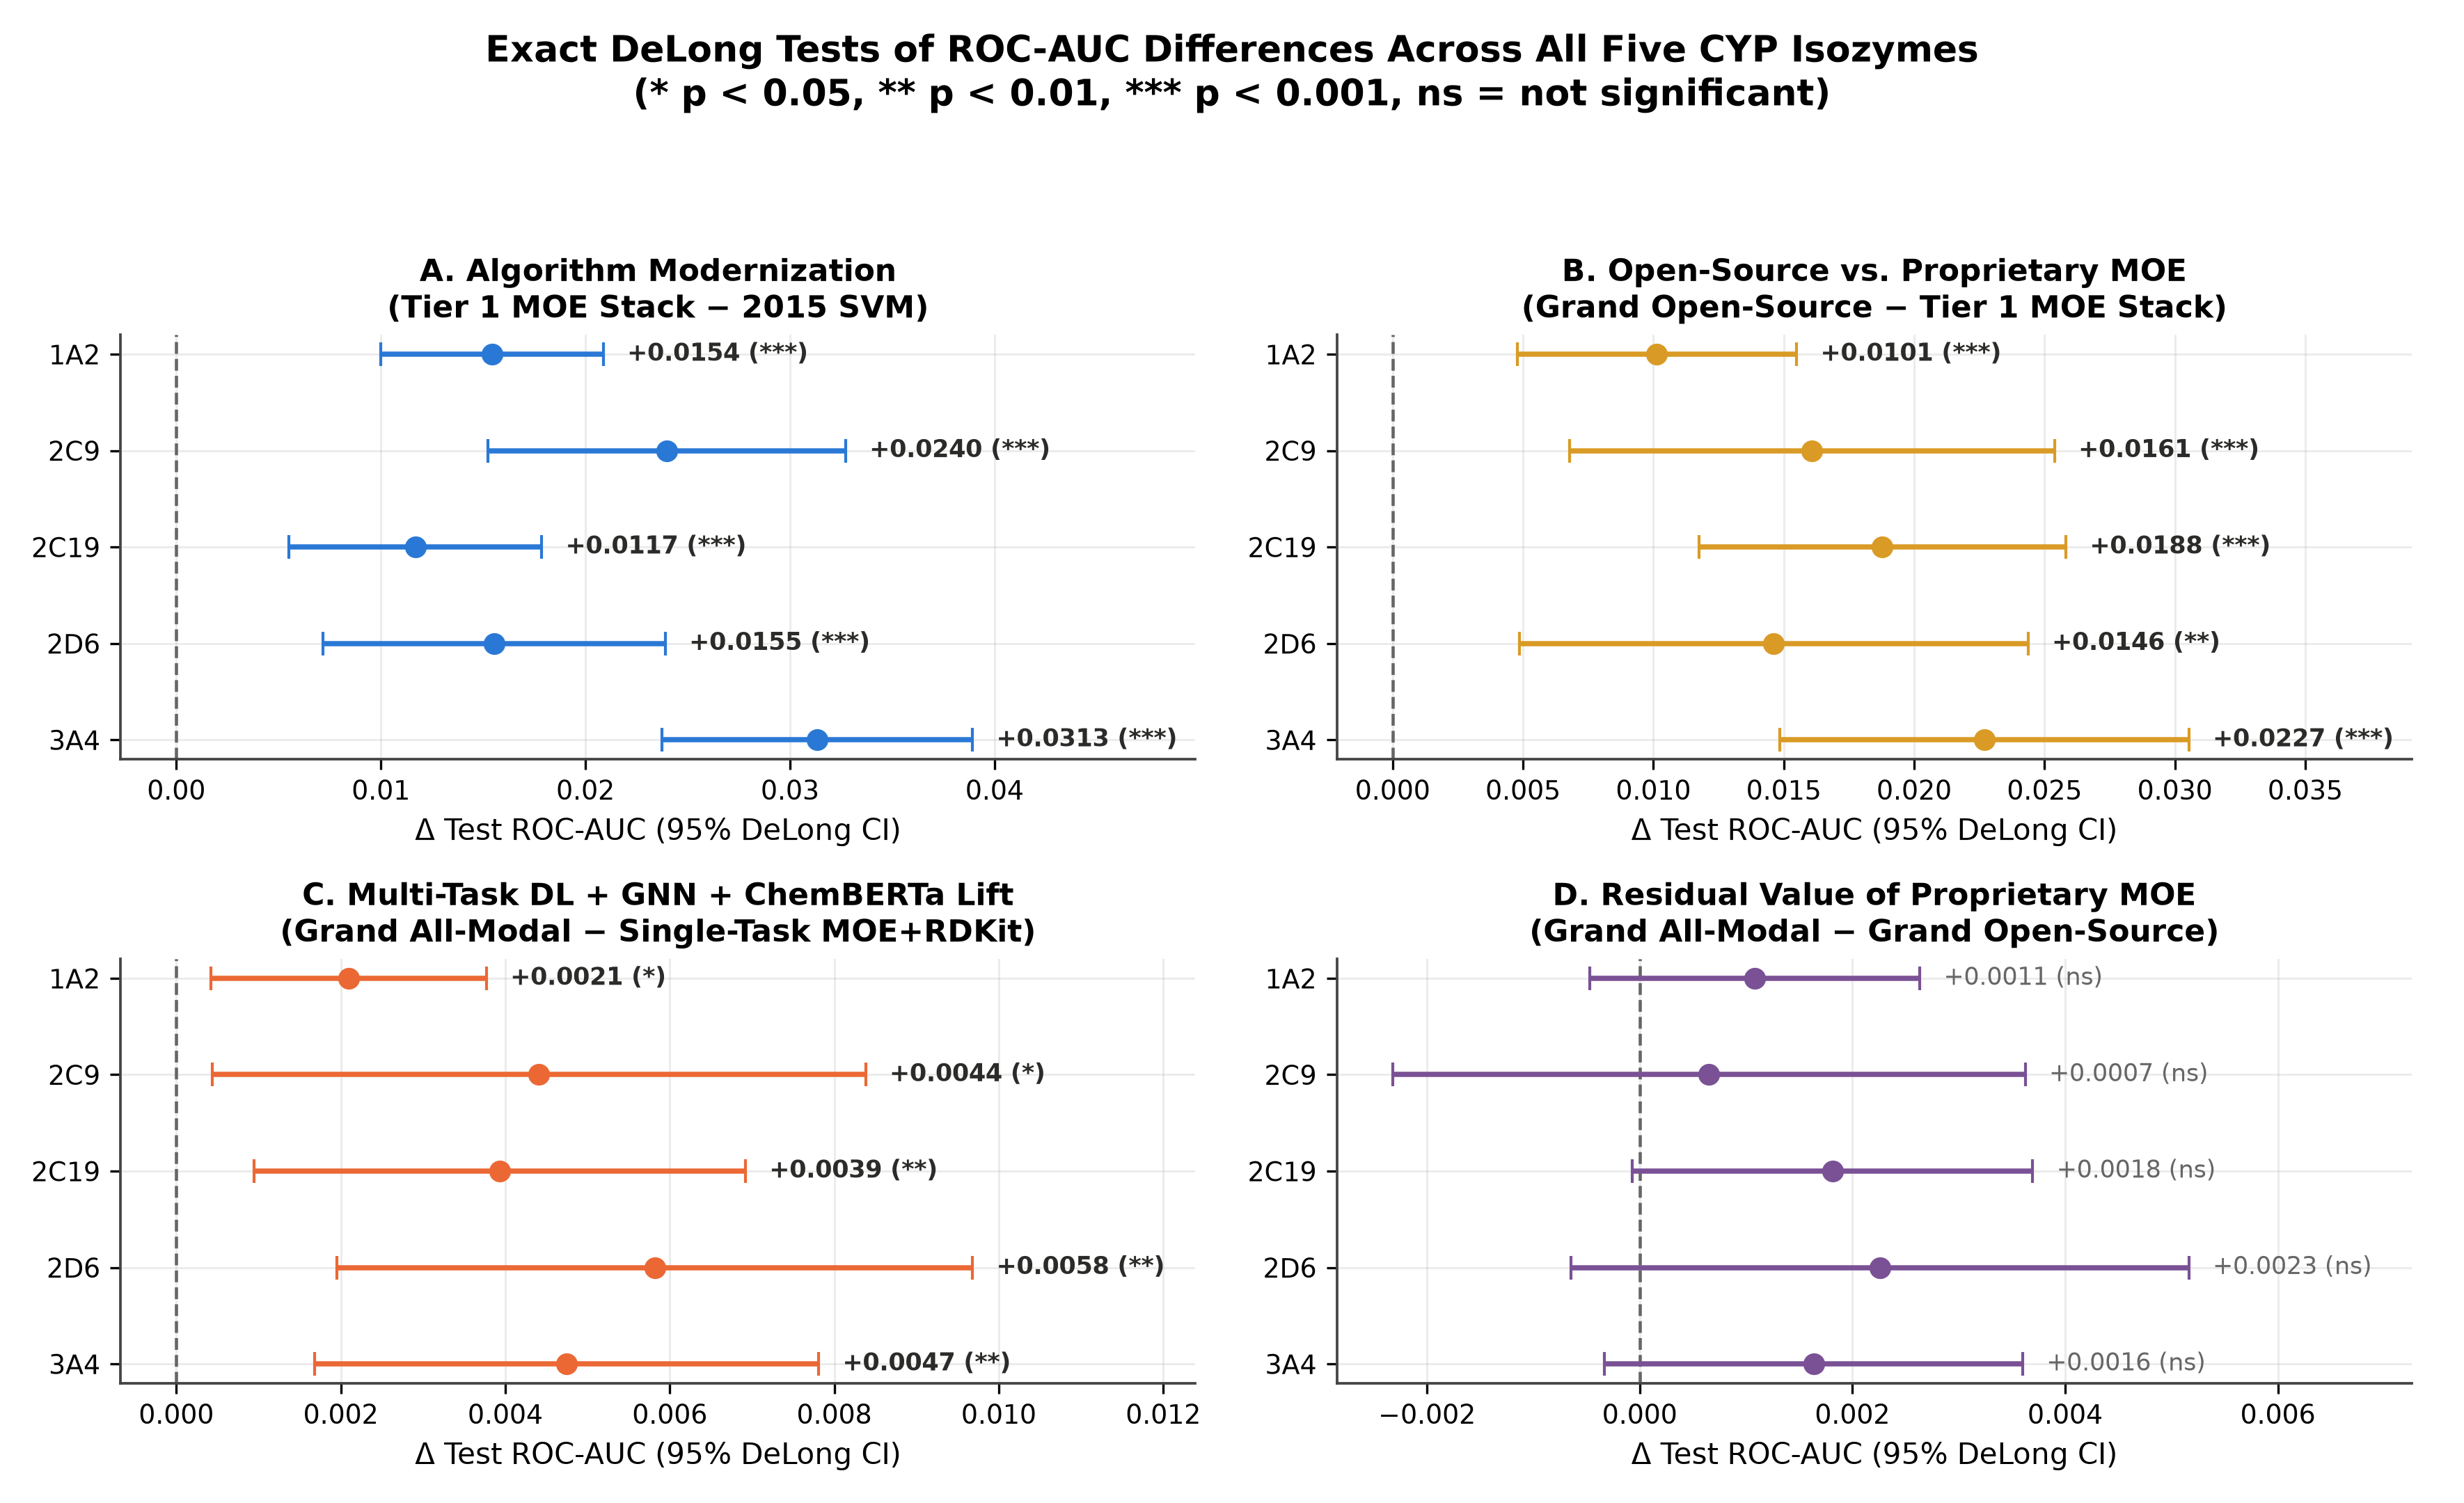
\includegraphics[width=0.93\textwidth]{../img/fig4_delong_forest.png}}\\[4pt]
{\scriptsize\sffamily\color{muted}\textbf{PLATE 2.} Exact Sun \& Xu (2014) DeLong forest plots. Look at Panel D: once open-source multi-modal ML enters the room, adding 186 proprietary MOE descriptors produces confidence intervals straddling zero on \textbf{all five isozymes} ($p \in [0.059, 0.668]$).}
\end{center}

\newpage
\section{Architecture, Synergy \& The Way of the Future}

\vspace{4pt}
\begin{center}
\fcolorbox{cobalt}{white}{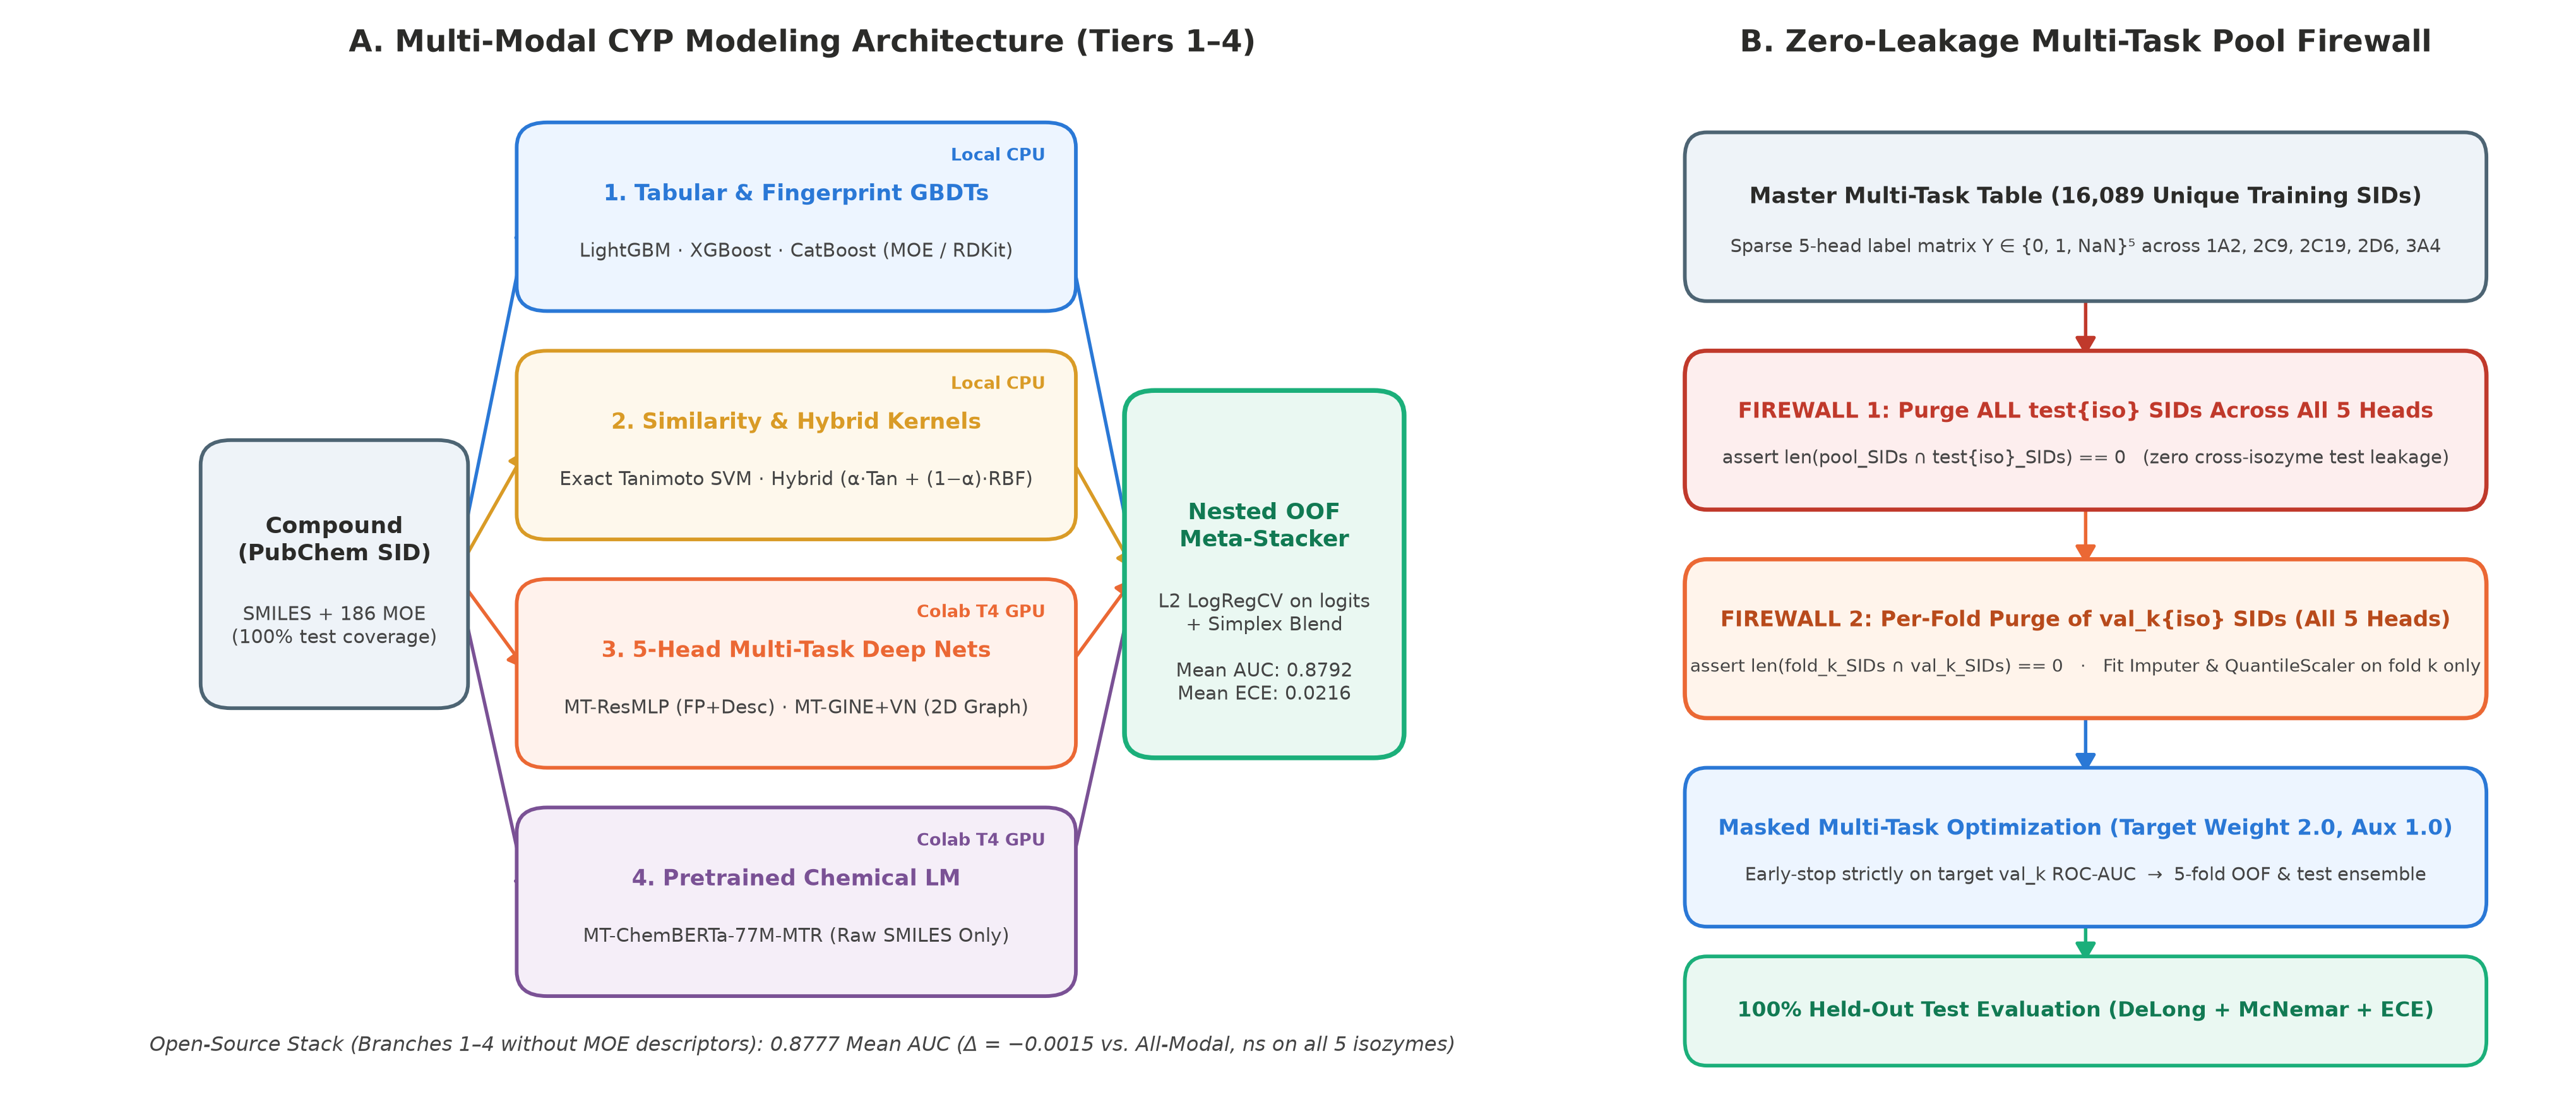
\includegraphics[width=0.90\textwidth]{../img/fig7_architecture_and_leakage.png}}\\[3pt]
{\scriptsize\sffamily\color{muted}\textbf{PLATE 3.} Four orthogonal modalities converging into a nested log-odds meta-stacker, guarded by a double-firewall multi-task SID purge.}
\end{center}

\vspace{4pt}
\begin{center}
\fcolorbox{violet}{white}{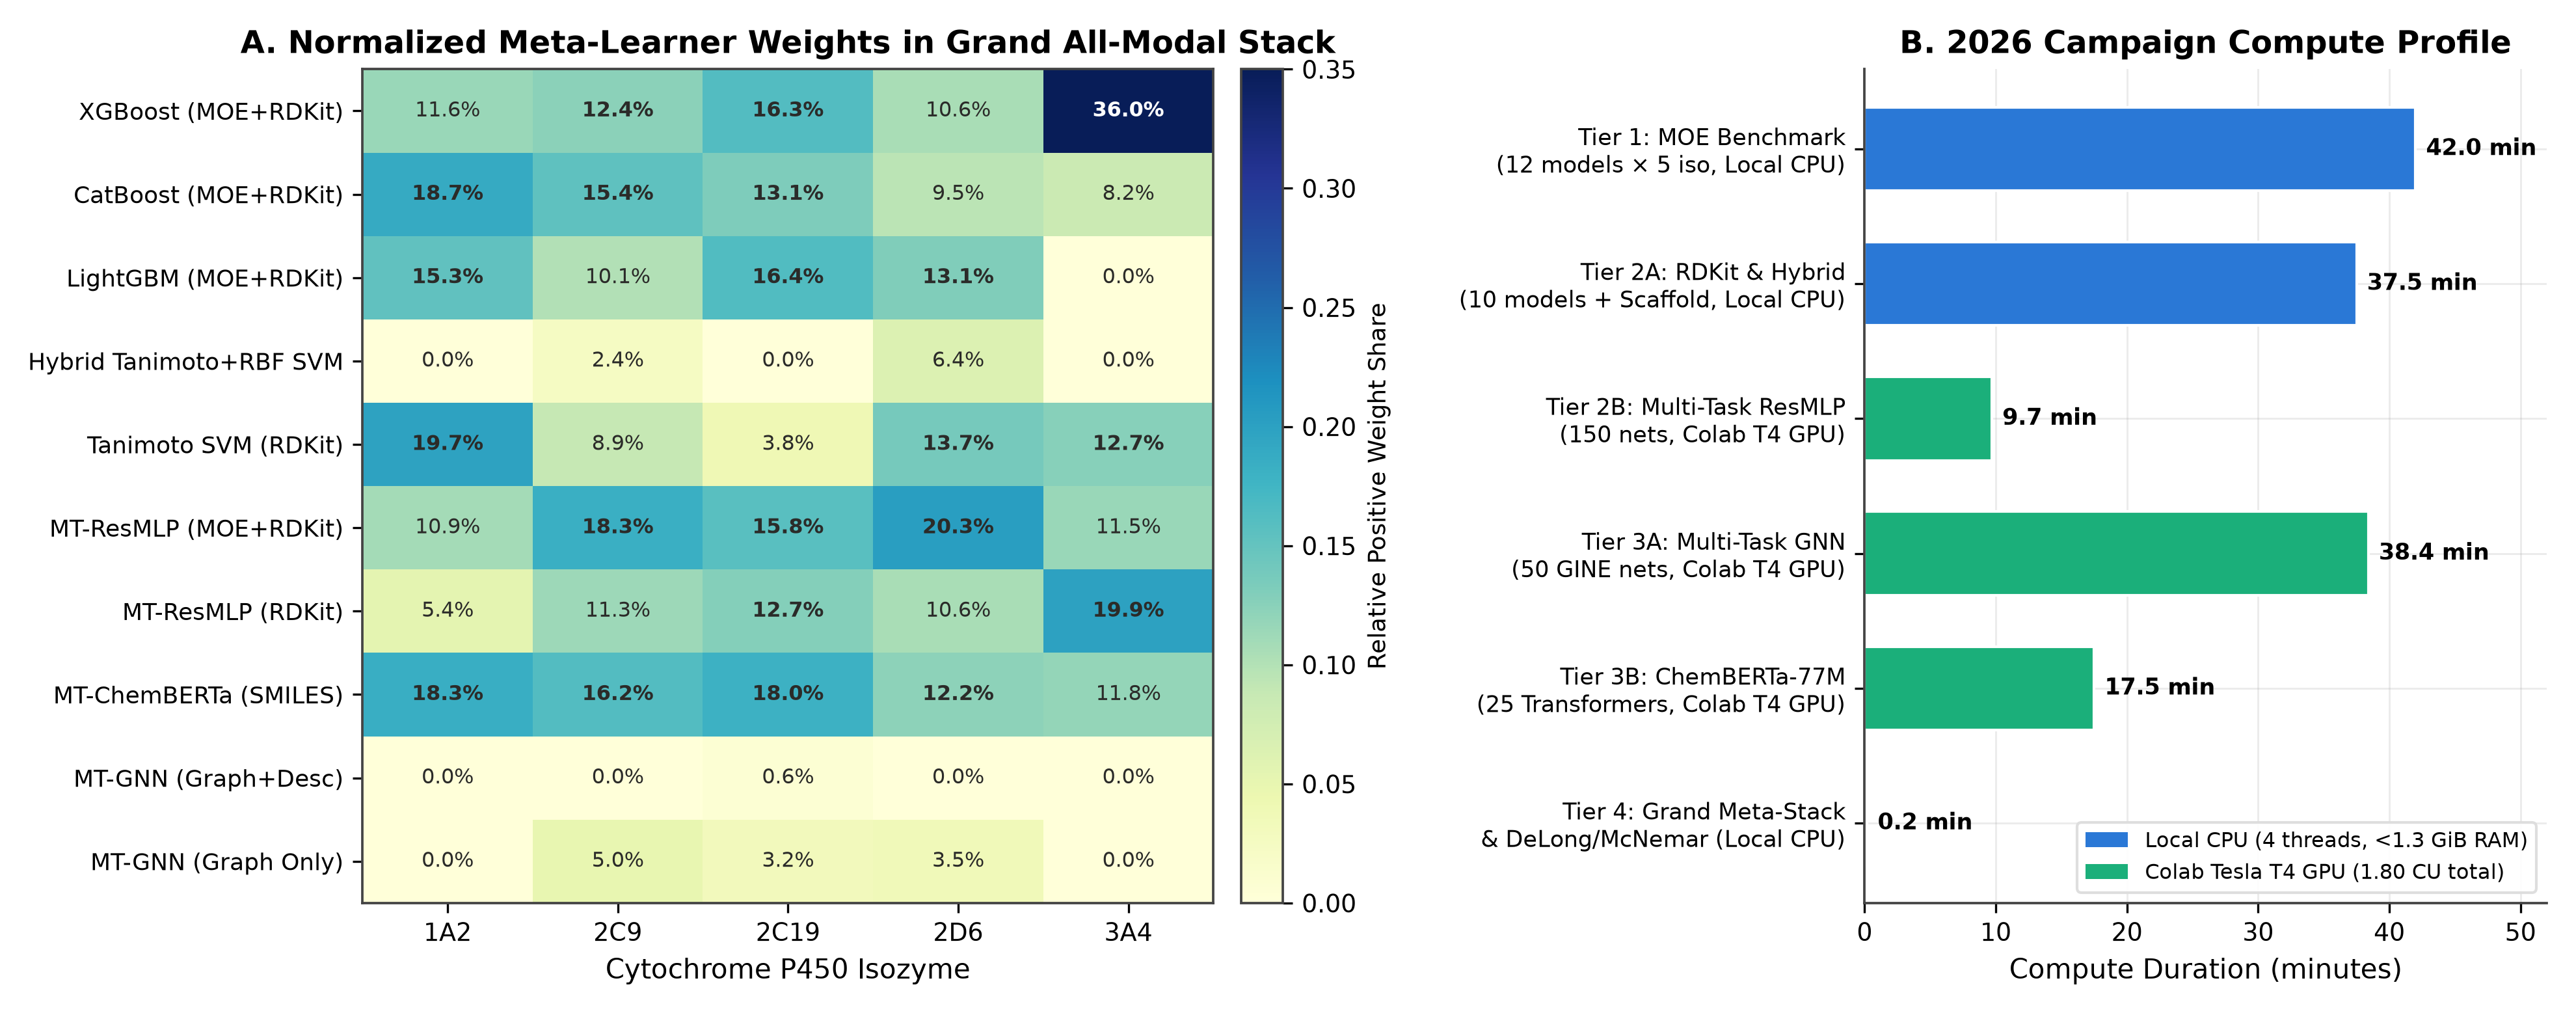
\includegraphics[width=0.90\textwidth]{../img/fig6_multimodal_weights_and_compute.png}}\\[3pt]
{\scriptsize\sffamily\color{muted}\textbf{PLATE 4.} Left: Every modality earns real weight in the Grand Stack (ChemBERTa pulls 12--18\% on every isozyme). Right: Entire 2026 campaign ran for 1.80 Colab T4 compute units.}
\end{center}

\vspace{4pt}
\begin{monolith}[emerald]{THE WAY OF THE FUTURE (2026--2035)}
\footnotesize
\textbf{\color{emerald}1. Static PDFs are fossils.} Companion interactive web paper at \texttt{extension/unhinged/index.html} lets readers scrub the 11-year Time Machine, slice all 5 isozymes live, and audit every DeLong test directly from verified CSV/NPZ archives.\\[3pt]
\textbf{\color{amber}2. The scientist is now a conductor.} The 2015 apprenticeship built the instincts---demanding 100\% test coverage, scaffold splits, and zero-leakage firewalls. In 2026, AI-coordinated hybrid compute turned an OOM crash into a $<$1.3\,GiB refactor in minutes, patched an fp16 CUDA scatter bug on the fly, and orchestrated $>1{,}000$ models across local CPU and cloud GPU in \textbf{3.5 wall-clock hours}.\\[3pt]
\textbf{\color{violet}3. Open weights eat proprietary silos.} World-class ADMET modeling no longer requires a five-figure commercial license---just open chemistry, open foundation models, a laptop, and two dollars of cloud GPU.
\end{monolith}

\end{document}
